\documentclass[12pt,a4paper]{report}

% Compile with: pdflatex PROJECT_TECHNICAL_FLOW.tex (run twice for the TOC).
\usepackage[utf8]{inputenc}
\usepackage[T1]{fontenc}
\usepackage{lmodern}
\usepackage[margin=1in]{geometry}
\usepackage{microtype}
\usepackage{amsmath,amssymb}
\usepackage{booktabs,longtable,array,tabularx}
\usepackage{enumitem}
\usepackage[dvipsnames,table]{xcolor}
\usepackage{graphicx}
\usepackage{float}
\usepackage{listings}
\usepackage{tikz}
\usetikzlibrary{arrows.meta,positioning,shapes.geometric,fit}
\usepackage[hidelinks]{hyperref}
\usepackage{cleveref}

\definecolor{Primary}{HTML}{0B5D56}
\definecolor{Secondary}{HTML}{315E8A}
\definecolor{Light}{HTML}{EAF4F2}
\definecolor{CodeBG}{HTML}{F4F6F8}
\definecolor{Muted}{HTML}{5B6770}

\hypersetup{
  pdftitle={Decoding Crime Narratives using NLP and Big Data Analytics},
  pdfauthor={Project Technical Documentation},
  pdfsubject={Objectives, theory, implementation and end-to-end system flow}
}

\setlist[itemize]{leftmargin=1.6em,itemsep=0.25em}
\setlist[enumerate]{leftmargin=1.8em,itemsep=0.35em}
\renewcommand{\arraystretch}{1.22}
\newcolumntype{Y}{>{\raggedright\arraybackslash}X}
\newcommand{\code}[1]{\texttt{#1}}
\newcommand{\project}{\textit{Decoding Crime Narratives using NLP and Big Data Analytics}}

\lstset{
  backgroundcolor=\color{CodeBG},
  basicstyle=\ttfamily\small,
  breaklines=true,
  frame=single,
  rulecolor=\color{gray!30},
  showstringspaces=false,
  columns=fullflexible,
  keepspaces=true
}

\tikzset{
  flow/.style={rectangle, rounded corners, draw=Primary, very thick,
    fill=Light, text width=4.2cm, minimum height=1.0cm, align=center},
  data/.style={cylinder, shape border rotate=90, aspect=0.22, draw=Secondary,
    very thick, fill=blue!7, text width=3.5cm, minimum height=1.05cm, align=center},
  arrow/.style={-{Latex[length=3mm]}, very thick, draw=Muted},
  note/.style={rectangle, draw=gray!55, dashed, fill=gray!5,
    text width=4.2cm, align=left, font=\small}
}

\begin{document}

\begin{titlepage}
  \centering
  \vspace*{1.2cm}
  {\Large\color{Primary}\textbf{Technical Project Report}\par}
  \vspace{0.8cm}
  {\Huge\bfseries Decoding Crime Narratives\par}
  \vspace{0.25cm}
  {\LARGE\bfseries using NLP and Big Data Analytics\par}
  \vspace{1.0cm}
  {\Large Objectives, Theory, Implementation, Data Flow and Functionalities\par}
  \vfill
  \begin{tabular}{rl}
    Project version: & 2.0.0 \\
    Dataset: & 60,000 clean fictional reports \\
    Main technologies: & Python, Apache Spark, scikit-learn, BERT, CRF, \\
                       & spaCy, NLTK, SQLite and Streamlit \\
    Reproducibility seed: & 42
  \end{tabular}
  \vfill
  {\large University NLP and Big Data Analytics Project\par}
  \vspace{0.5cm}
  {\large \today\par}
\end{titlepage}

\pagenumbering{roman}
\tableofcontents
\clearpage
\listoffigures
\clearpage
\pagenumbering{arabic}

\chapter{Objective and Purpose}

\section{Main objective}

The objective of \project{} is to build a reproducible, end-to-end system that converts a large collection of unstructured English crime narratives into structured, searchable and explainable information. The system demonstrates how concepts from Natural Language Processing (NLP), machine learning and Big Data Analytics can be connected in one working pipeline.

For an input narrative, the system aims to answer the following questions:

\begin{itemize}
  \item What broad crime category does the narrative resemble?
  \item Which phrases refer to a suspect, victim, location, weapon, property, date, time or item of evidence?
  \item What are the important grammatical relations in the sentences?
  \item What is the polarity of the language, and which explicit threat-related words occur?
  \item Which recurring topic best represents the narrative?
  \item Which source sentences form a short extractive summary?
  \item Which stored reports are relevant to a keyword or natural-language query?
  \item How accurate are the trained models under the project's fixed synthetic evaluation protocol?
\end{itemize}

\section{Purpose of the project}

The project has four connected purposes.

\begin{enumerate}
  \item \textbf{Educational purpose:} demonstrate document representation, classification, sequence labelling, topic modelling, syntax, sentiment, summarisation, retrieval and evaluation.
  \item \textbf{Big Data purpose:} demonstrate schema-based ingestion, partitioned execution, cleaning, deterministic deduplication, SQL aggregation, Parquet storage and an MLlib pipeline using Apache Spark.
  \item \textbf{Engineering purpose:} connect data generation, processing, model training, model freezing, enrichment, indexing, disk-backed storage, testing and a dashboard through reproducible artifacts.
  \item \textbf{Research purpose:} compare classical and neural approaches under the same data protocol while reporting limitations instead of assuming that the most complex model must be best.
\end{enumerate}

\section{Intended and prohibited interpretations}

All persons, places and incidents in the main corpus are fictional. The project is intended for university demonstration and controlled experimentation. It must not be interpreted as a real crime-rate database, a system for determining guilt, or a validated danger-prediction system. A model-produced label is a suggestion based on language patterns, not a legal conclusion.

\chapter{Complete System Flow}

\section{End-to-end pipeline}

\begin{figure}[H]
\centering
\resizebox{0.96\textwidth}{!}{%
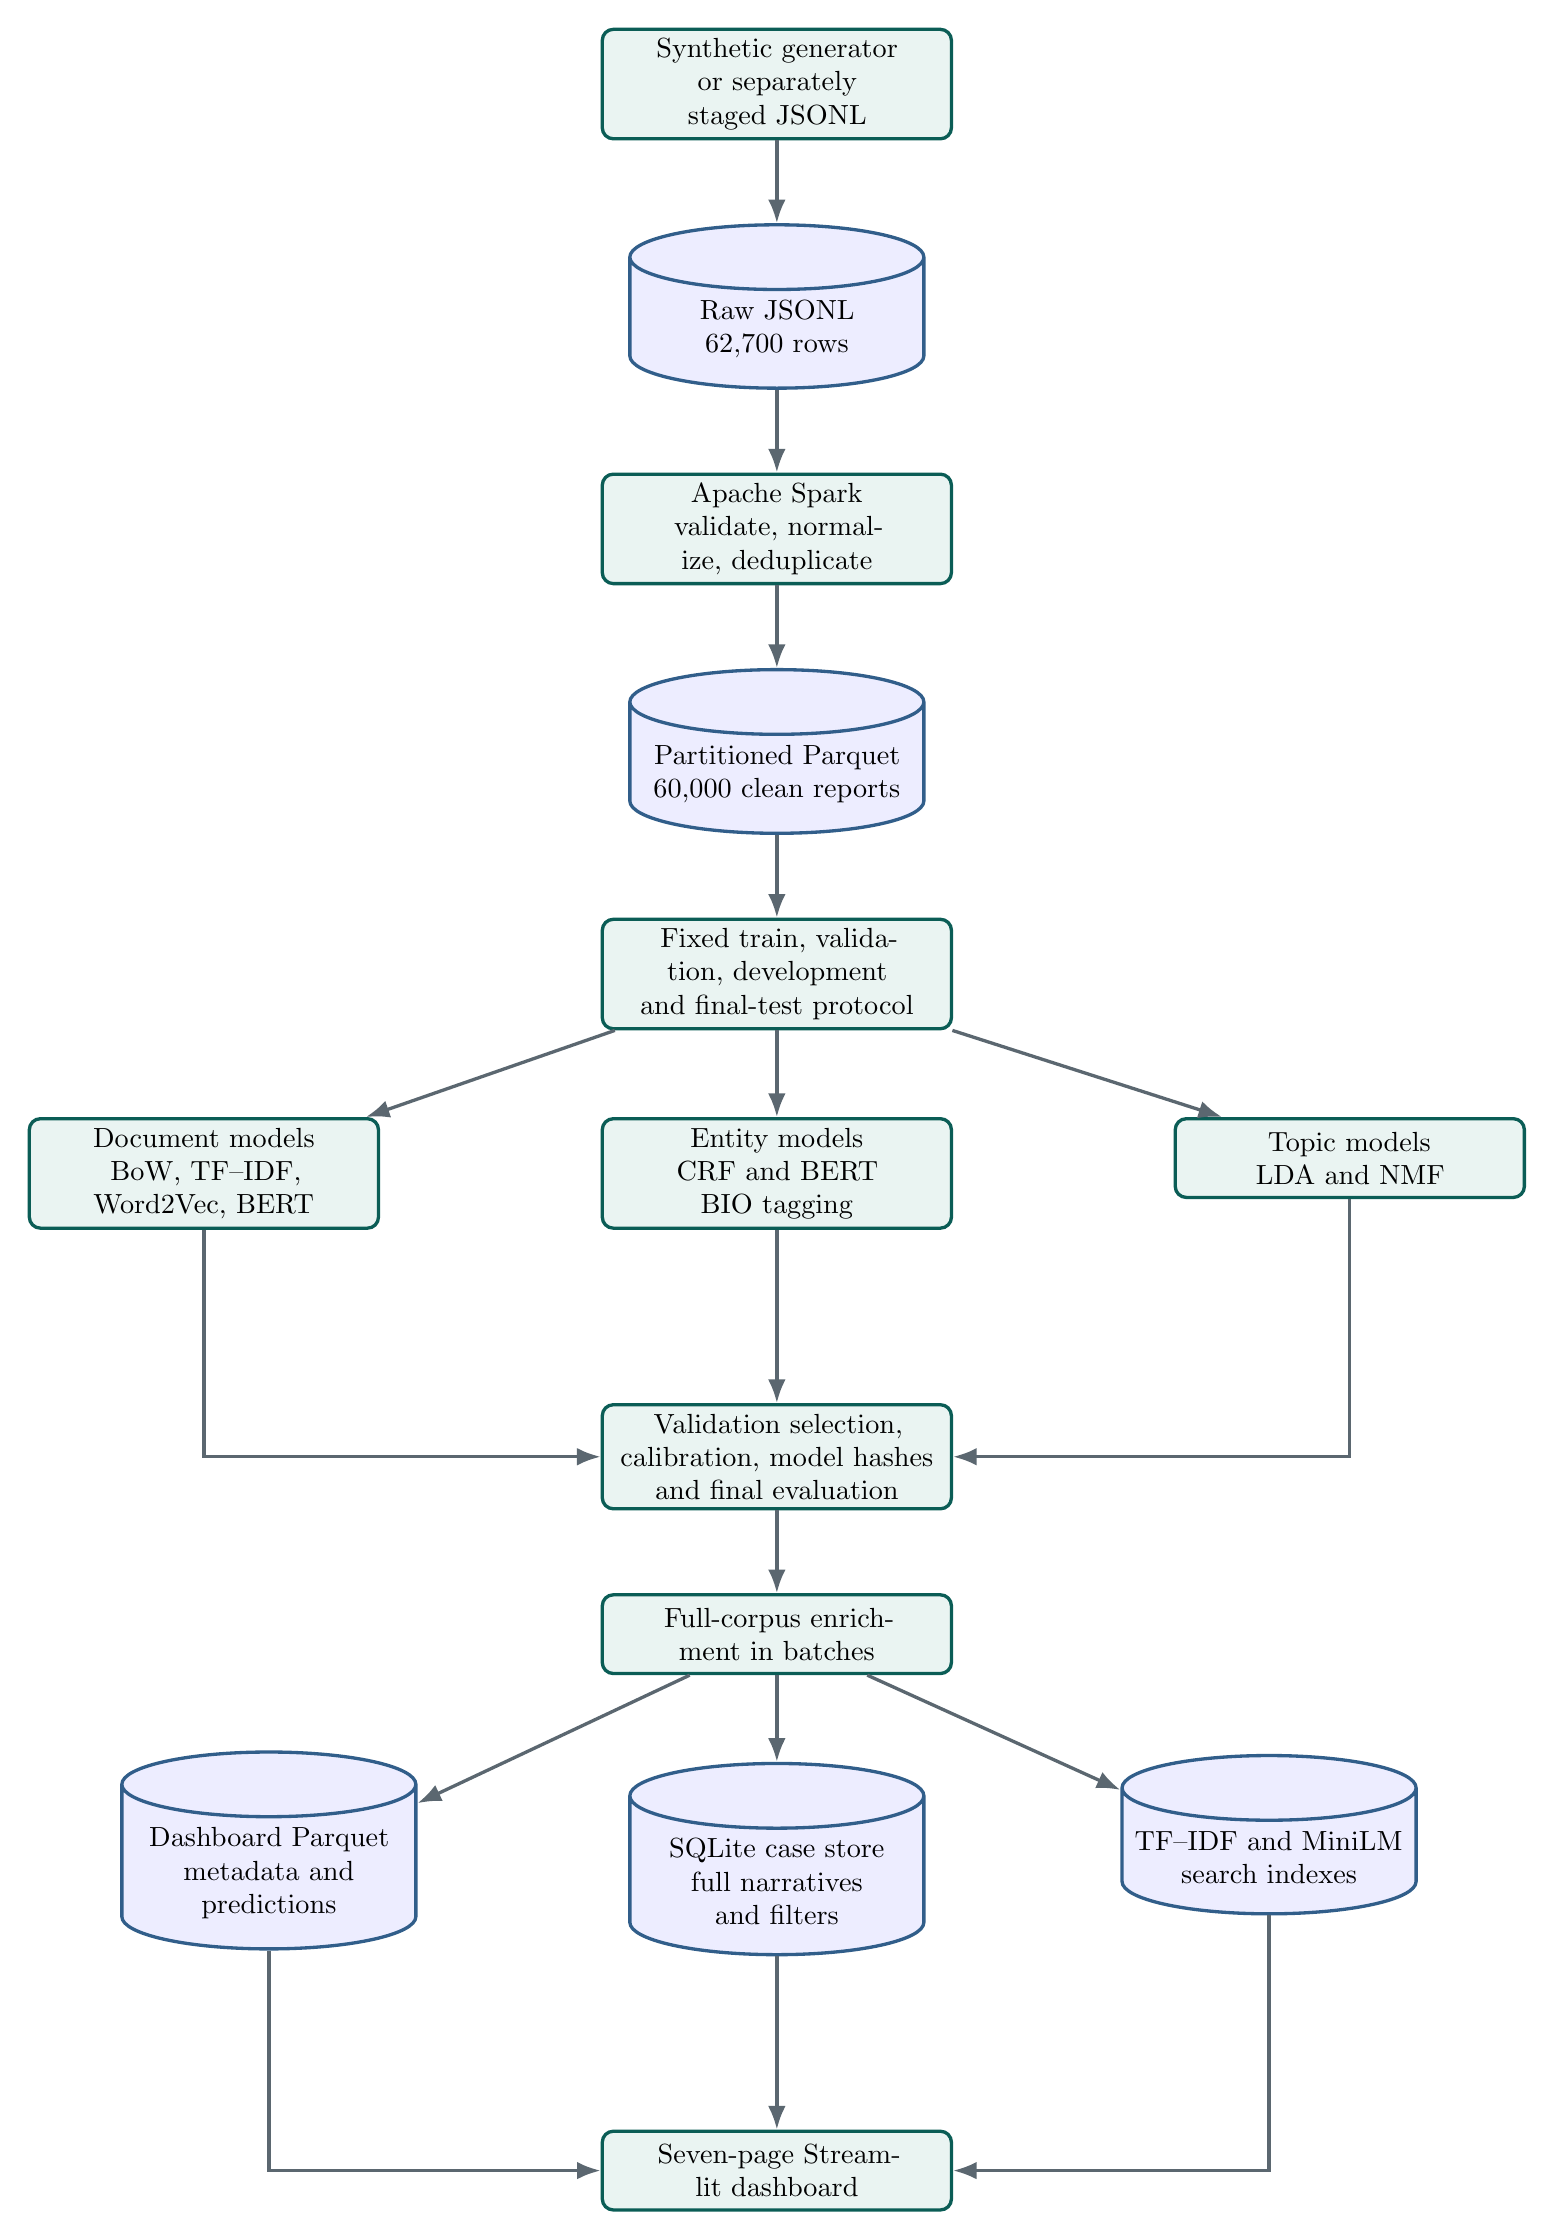
\begin{tikzpicture}[node distance=1.05cm]
  \node[flow] (source) {Synthetic generator\\or separately staged JSONL};
  \node[data, below=of source] (raw) {Raw JSONL\\62,700 rows};
  \node[flow, below=of raw] (spark) {Apache Spark\\validate, normalize, deduplicate};
  \node[data, below=of spark] (parquet) {Partitioned Parquet\\60,000 clean reports};
  \node[flow, below=of parquet] (split) {Fixed train, validation, development and final-test protocol};
  \node[flow, below left=1.1cm and 2.8cm of split] (doc) {Document models\\BoW, TF--IDF, Word2Vec, BERT};
  \node[flow, below=1.1cm of split] (ner) {Entity models\\CRF and BERT BIO tagging};
  \node[flow, below right=1.1cm and 2.8cm of split] (topic) {Topic models\\LDA and NMF};
  \node[flow, below=2.2cm of ner] (freeze) {Validation selection, calibration, model hashes and final evaluation};
  \node[flow, below=of freeze] (enrich) {Full-corpus enrichment in batches};
  \node[data, below left=1.1cm and 2.8cm of enrich] (dashdata) {Dashboard Parquet\\metadata and predictions};
  \node[data, below=1.1cm of enrich] (sqlite) {SQLite case store\\full narratives and filters};
  \node[data, below right=1.1cm and 2.8cm of enrich] (indexes) {TF--IDF and MiniLM\\search indexes};
  \node[flow, below=2.2cm of sqlite] (ui) {Seven-page Streamlit dashboard};

  \draw[arrow] (source) -- (raw);
  \draw[arrow] (raw) -- (spark);
  \draw[arrow] (spark) -- (parquet);
  \draw[arrow] (parquet) -- (split);
  \draw[arrow] (split) -- (doc);
  \draw[arrow] (split) -- (ner);
  \draw[arrow] (split) -- (topic);
  \draw[arrow] (doc) |- (freeze);
  \draw[arrow] (ner) -- (freeze);
  \draw[arrow] (topic) |- (freeze);
  \draw[arrow] (freeze) -- (enrich);
  \draw[arrow] (enrich) -- (dashdata);
  \draw[arrow] (enrich) -- (sqlite);
  \draw[arrow] (enrich) -- (indexes);
  \draw[arrow] (dashdata) |- (ui);
  \draw[arrow] (sqlite) -- (ui);
  \draw[arrow] (indexes) |- (ui);
\end{tikzpicture}}
\caption{End-to-end flow from source data to the interactive dashboard.}
\label{fig:end-to-end}
\end{figure}

\section{Pipeline controller}

The file \path{run_pipeline.py} is the orchestration layer. Its command-line argument \code{--stage} selects \code{generate}, \code{spark}, \code{train}, \code{enrich}, or all stages in order. Each stage is treated as a producer of artifacts consumed by later stages.

\begin{longtable}{p{0.16\textwidth}p{0.32\textwidth}p{0.42\textwidth}}
\toprule
\textbf{Stage} & \textbf{Main responsibility} & \textbf{Important outputs} \\
\midrule
\endhead
Generate & Produce reproducible fictional narratives and exact entity annotations; inject controlled data faults. & \path{data/raw/reports.jsonl}, \path{artifacts/dataset_manifest.json} \\
Spark & Validate schema and values, normalize text, remove duplicates, create aggregates and train a distributed baseline. & Partitioned report Parquet, trends, quality report, physical execution plan and MLlib model \\
Train & Fit document, entity and topic models; select checkpoints; calibrate; freeze; evaluate. & Joblib models, BERT checkpoints, evaluation JSON, error CSV, topic and NER results \\
Enrich & Apply selected models to all clean reports and build the stores required by the dashboard. & Dashboard Parquet, SQLite, sparse keyword index and dense semantic index \\
\bottomrule
\end{longtable}

The optional \code{--resume} mode uses SHA--256 signatures. A stage can be reused only when its arguments, relevant source files, inputs and recorded outputs still match. This protects the user from unknowingly combining stale downstream files with changed upstream code or data.

\chapter{Data Project: Generation, Annotation and Ingestion}

\section{Synthetic corpus design}

The project uses a deterministic generator because a university demonstration requires enough labelled data for every pipeline stage without exposing private real-world records. A fixed pseudo-random seed of 42 makes the generation repeatable.

The corpus contains eight balanced document categories: Arson, Assault, Burglary, Cybercrime, Fraud, Robbery, Theft and Vandalism. Each category has eight event variants and each report is arranged using one of six layouts, giving

\begin{equation}
8\ \text{categories} \times 8\ \text{event variants} \times 6\ \text{layouts}
=384\ \text{composite scenario groups}.
\end{equation}

Additional variation includes different fictional names, districts, locations, property, weapons, evidence, multiple participants, unknown suspects, negated weapon mentions, spelling noise and longer follow-up paragraphs.

\section{Record schema}

Each JSONL line is one JSON object. The key fields are shown in \cref{tab:schema}.

\begin{longtable}{p{0.22\textwidth}p{0.68\textwidth}}
\caption{Principal fields in a generated report.}\label{tab:schema}\\
\toprule
\textbf{Field} & \textbf{Purpose} \\
\midrule
\endfirsthead
\toprule
\textbf{Field} & \textbf{Purpose} \\
\midrule
\endhead
\code{report\_id} & Stable identifier used through the complete pipeline. \\
\code{narrative} & Original human-readable text. It remains unchanged so that entity offsets continue to point to the correct characters. \\
\code{crime\_type} & Generator-produced reference label for document classification. \\
\code{reported\_at} & ISO-formatted fictional date and time. \\
\code{district} & Fictional geographical grouping used in filters and aggregates. \\
\code{template\_group} & Category, event variant and layout family used to prevent group leakage. \\
\code{split} & Training, validation, development or final-test partition. \\
\code{source} & Provenance marker, \code{synthetic-v2}. \\
\code{entities\_json} & Exact start/end character offsets, surface text and label for every generated entity. \\
\bottomrule
\end{longtable}

\section{Exact span annotation}

While a template is rendered, the generator tracks the running character position. If a placeholder contains an entity, it records

\begin{equation}
e=(s,e,\ell,t),
\end{equation}

where $s$ is the inclusive start offset, $e$ is the exclusive end offset, $\ell$ is the entity type and $t$ is the exact substring. The invariant

\begin{equation}
\texttt{narrative}[s:e]=t
\end{equation}

is tested across all template layouts. These automatically generated spans act as the reference annotations for NER evaluation; they are not human annotations.

\section{Controlled data-quality faults}

The generator writes 60,000 valid unique records and then injects 2,700 controlled faults:

\begin{center}
\begin{tabular}{lr}
\toprule
Condition & Rows \\
\midrule
Duplicates & 1,500 \\
Null narratives & 600 \\
Blank narratives & 300 \\
Invalid dates & 300 \\
\midrule
Total raw input & 62,700 \\
\bottomrule
\end{tabular}
\end{center}

The faults provide measurable cleaning requirements. The expected clean output is exactly 60,000 records.

\section{Split design}

For each category, variants 0--4 belong to training, variant 5 to validation, variant 6 to development, and variant 7 to final test. First-name pools and participant phrasings are also split-specific. The purpose is to make direct memorisation less useful.

\begin{itemize}
  \item \textbf{Training} estimates model parameters.
  \item \textbf{Validation} chooses checkpoints, selects the entity model and fits confidence calibration.
  \item \textbf{Development} provides additional diagnostics without opening the final test.
  \item \textbf{Final test} measures frozen models after hashes have been recorded.
\end{itemize}

The grammar and much of the vocabulary are still shared because all records come from one generator. The split reduces specific leakage but cannot simulate a truly independent real-world source.

\section{External JSONL staging}

The optional file \path{scripts/import_jsonl.py} calls \path{crime_nlp/import_data.py}. It validates required IDs, UTF--8 text, ISO dates, optional category values, non-overlapping spans and exact span text. It records a source URL, licence description and SHA--256 digest. Invalid rows and duplicate IDs are quarantined without copying their raw narrative text into error reports.

External records remain in a separate staging location; they are not silently mixed with the synthetic benchmark. A genuine external experiment would require permission, reviewed labels, a mapping to project categories and a new split protocol.

\chapter{Big Data Project: Apache Spark Processing}

\section{Why Apache Spark is used}

Spark represents tabular data using distributed DataFrames. A driver constructs a logical plan; executors run tasks over partitions. Transformations such as \code{filter} are lazy, while actions such as \code{count} and \code{write} trigger execution.

The project uses Spark to demonstrate that large-scale cleaning is expressed as a partitioned computation rather than as an ordinary row-by-row loop. On the verified machine, the standalone demonstration used one Spark master and two independent worker processes on one physical host. This demonstrates process-level distributed execution but is not a multi-host performance benchmark.

\section{Spark cleaning sequence}

The implementation is in \path{crime_nlp/spark_pipeline.py}. Its operations are:

\begin{enumerate}
  \item Read raw JSON with an explicit all-string schema.
  \item Repartition the DataFrame into eight partitions.
  \item Drop rows missing required fields.
  \item Reject narratives that are empty after trimming.
  \item Parse \code{reported\_at} into a Spark timestamp.
  \item Reject invalid dates, categories and split names.
  \item Preserve \code{narrative}; create a separate lowercase \code{clean\_text} column.
  \item Replace punctuation with spaces and collapse repeated whitespace in \code{clean\_text}.
  \item Compute a SHA--256 \code{text\_hash} from normalized text.
  \item Use a window ordered by \code{report\_id} to keep one deterministic canonical row per hash.
  \item Derive the month used by the dashboard's temporal visualisations.
  \item Write Parquet partitioned by \code{split}.
  \item Run Spark SQL grouping by month, category and district.
\end{enumerate}

Deterministic deduplication is important. A plain unordered duplicate removal can choose different surviving identifiers in different executions. The row-number window makes the survivor rule explicit.

\section{Parquet contribution}

Parquet is a columnar format. Columns are stored together, so an analytical reader can load selected columns without scanning every full narrative. Partitioning by split also allows processing to skip unrelated directory partitions. In this system, Parquet is the main analytical and model-training store.

\section{Distributed MLlib baseline}

The Spark ML pipeline is

\iffalse

\begin{equation}
\text{RegexTokenizer}
ightarrow\text{StopWordsRemover}
ightarrow
\text{HashingTF}
ightarrow\text{IDF}
ightarrow\text{LogisticRegression}.
\end{equation}
\fi

\begin{equation}
\text{RegexTokenizer}
\rightarrow\text{StopWordsRemover}
\rightarrow\text{HashingTF}
\rightarrow\text{IDF}
\rightarrow\text{LogisticRegression}.
\end{equation}

\textbf{HashingTF} maps tokens into a fixed 4,096-dimensional feature space using a hash function. IDF reduces the influence of widely occurring terms. Multinomial logistic regression estimates a probability distribution over eight categories. The saved Spark model obtained approximately 87.49\% accuracy and 83.35\% weighted F1 on the full held-out Spark test partition.

\chapter{Text Representation and Document Classification}

\section{General supervised-learning formulation}

For reports $(x_i,y_i)$, $x_i$ is the narrative and $y_i$ is one of eight categories. A representation function $\phi(x_i)$ converts text into a numeric vector. A classifier then estimates

\begin{equation}
\hat{y}_i=\arg\max_{c\in\mathcal{C}} P(y=c\mid\phi(x_i)).
\end{equation}

The project compares four representations under the same sampled split protocol: Bag of Words, TF--IDF, averaged Word2Vec and compact BERT.

\section{Bag of Words}

Bag of Words represents document $d$ by term counts:

\begin{equation}
x_{d,t}=\operatorname{count}(t,d).
\end{equation}

The implementation uses \code{CountVectorizer} with unigrams and bigrams, a maximum of 12,000 features and a minimum document frequency of two. Word order is ignored beyond the local bigrams, but the representation is fast and interpretable.

The resulting sparse vector is passed to multinomial logistic regression. For category $c$,

\begin{equation}
P(y=c\mid x)=\frac{\exp(w_c^Tx+b_c)}{\sum_k\exp(w_k^Tx+b_k)}.
\end{equation}

Its final synthetic-test accuracy is 78.42\%.

\section{TF--IDF}

Term frequency--inverse document frequency emphasizes terms that are frequent in one document but less frequent in the corpus. A standard form is

\begin{align}
\operatorname{tf}(t,d)&=\operatorname{count}(t,d),\\
\operatorname{idf}(t)&=\log\frac{N+1}{\operatorname{df}(t)+1}+1,\\
\operatorname{tfidf}(t,d)&=\operatorname{tf}(t,d)\operatorname{idf}(t).
\end{align}

The project uses unigrams and bigrams, 12,000 maximum features, minimum document frequency two and sublinear term frequency. Logistic regression performs classification. Its final accuracy is 83.67\%.

TF--IDF is the dashboard default even though it is not the highest-scoring model. It provides fast CPU inference, compact storage and a direct feature-contribution explanation. For predicted class $c$, the displayed contribution of feature $j$ is approximately

\begin{equation}
\text{contribution}_{j,c}=x_jw_{c,j}.
\end{equation}

This is an explanation of the linear score, not proof of causality.

\section{Word2Vec document classification}

Word2Vec learns dense word vectors by predicting local context. The project uses the skip-gram architecture, a 100-dimensional vector, a context window of five, twelve training epochs and one worker for reproducibility.

If $V_d$ is the set of in-vocabulary words in document $d$, the document vector is

\begin{equation}
v_d=\frac{1}{|V_d|}\sum_{w\in V_d}v_w.
\end{equation}

Logistic regression is fitted on the averaged document vectors. This loses detailed order but captures distributional similarity between terms. Its final accuracy is 95.17\%, the highest document score in this executed experiment.

\section{BERT sequence classification}

BERT is a bidirectional Transformer. Self-attention allows each token representation to incorporate contextual information from other positions:

\begin{equation}
\operatorname{Attention}(Q,K,V)=\operatorname{softmax}\left(\frac{QK^T}{\sqrt{d_k}}\right)V.
\end{equation}

The implementation fine-tunes \code{google/bert\_uncased\_L-2\_H-128\_A-2}, containing two Transformer layers, hidden size 128 and two attention heads. Narratives are padded or truncated to 160 subtokens. AdamW optimization uses a learning rate of $5\times10^{-4}$, weight decay 0.01, gradient clipping and deterministic seeding.

After each epoch, validation macro-F1 is measured; only the best validation checkpoint is retained. Its final accuracy is 83.25\%. This result demonstrates that a neural Transformer is not automatically superior when the model is compact, training is bounded and the corpus has strong lexical/template structure.

\section{Grouped cross-validation}

Within the training partition, the TF--IDF model is also evaluated with three-fold \code{GroupKFold}. Groups are incident variants rather than individual rows. Related layouts remain together, preventing the cross-validation learner from seeing another layout of the same grouped incident in its training fold. The low recorded mean macro-F1 of about 0.2502 indicates that some held-out variant groups are much harder than the fixed final split.

\chapter{Probability Calibration and Evaluation Protocol}

\section{Temperature scaling}

Classification probabilities can be poorly calibrated even when category accuracy is acceptable. Let $p_c$ be an original class probability. The system converts it to a log score, divides by temperature $T$, and re-normalizes:

\begin{equation}
\tilde{p}_c=\frac{\exp(\log(p_c)/T)}{\sum_k\exp(\log(p_k)/T)}.
\end{equation}

$T$ is chosen on validation data by minimizing multiclass log loss. Because division by a positive temperature preserves score order, the predicted class does not change; only confidence sharpness changes.

The configured review threshold is 0.60. Scores below it produce \code{review\_required=true}. On the final synthetic test, temperature scaling reduced expected calibration error from about 0.3830 to 0.0757. Calibrated coverage was 92.17\%, and accuracy among accepted predictions was 85.80\%.

\section{Classification metrics}

For a class, precision, recall and F1 are

\begin{align}
\operatorname{Precision}&=\frac{TP}{TP+FP},\\
\operatorname{Recall}&=\frac{TP}{TP+FN},\\
F_1&=2\frac{\operatorname{Precision}\cdot\operatorname{Recall}}
{\operatorname{Precision}+\operatorname{Recall}}.
\end{align}

Macro-F1 averages class F1 values equally. Weighted-F1 weights them by class support. A confusion matrix records reference labels by predicted labels. The project also computes a 95\% report-level bootstrap interval from 400 resamples. That interval represents resampling variability within the synthetic test, not uncertainty caused by new cities, sources or writing styles.

\section{Freeze-before-test protocol}

Validation-driven choices are completed first. SHA--256 hashes of every model file are then stored in \path{artifacts/frozen_models.json}. Only afterward are final-test predictions produced and a final-evaluation receipt written. This creates evidence that the reported final evaluation refers to fixed files. Once final results have influenced future choices, a new independent protocol is required for the next release.

\chapter{Named Entity Recognition Project}

\section{Task and contribution}

Named Entity Recognition converts unstructured mentions into typed spans. The project supports SUSPECT, VICTIM, LOCATION, WEAPON, PROPERTY, DATE, TIME and EVIDENCE. These spans enable highlighting, filtering, structured summaries, negation handling and redaction.

\section{BIO sequence representation}

Tokens are assigned tags from the BIO scheme:

\begin{itemize}
  \item \code{B-TYPE}: beginning of an entity;
  \item \code{I-TYPE}: continuation of the same entity;
  \item \code{O}: not part of a target entity.
\end{itemize}

For example, ``Ari Mehra carried a knife'' becomes \code{B-VICTIM}, \code{I-VICTIM}, \code{O}, \code{O}, \code{B-WEAPON}. At inference time, adjacent BIO tags are converted back into exact character spans. An illegal orphan \code{I-TYPE} is repaired to \code{B-TYPE}.

\section{Conditional Random Field}

A linear-chain CRF scores an entire label sequence:

\begin{equation}
s(x,y)=\sum_{i=1}^{n}w^Tf(y_i,x,i)+\sum_{i=2}^{n}A_{y_{i-1},y_i},
\end{equation}

and predicts the sequence with maximum score. Unlike independent token classification, transition scores model the compatibility of adjacent labels.

The CRF observations include lowercase form, suffixes, capitalization, digits, punctuation, neighbouring words, document boundaries and sentence-level role cues. It is trained with L-BFGS, $c_1=c_2=0.1$, 100 maximum iterations and all possible label transitions.

\section{BERT token classification}

The BERT NER model assigns a BIO distribution to every input subtoken. Since reference labels are word-based, only the first subtoken of a word contributes to training loss; later subtokens receive the ignore value $-100$.

Long inputs are handled through overlapping 48-word windows with a stride of 32. Scores from overlapping windows are averaged for each original word. Exceptionally subword-heavy windows are recursively divided so that no original word is silently discarded.

The model uses AdamW, learning rate $3\times10^{-4}$, weight decay 0.01, gradient clipping and five epochs. The checkpoint with the best validation strict span F1 is saved.

\section{Model selection and results}

Strict entity F1 requires an exact boundary and correct type. Finding only ``Ari'' when the reference is ``Ari Mehra'' is incorrect. Automatic NER uses the model with higher validation strict F1; ties choose the faster CRF.

\begin{center}
\begin{tabular}{lrr}
\toprule
Model & Validation strict F1 & Final strict F1 \\
\midrule
CRF & 1.0000 & 0.9846 \\
BERT token classifier & 0.9414 & 0.8741 \\
\bottomrule
\end{tabular}
\end{center}

CRF is therefore selected. However, its PROPERTY recall is only 0.44 and PROPERTY F1 is 0.6111. Easier, frequent types dominate the overall score, showing why per-type evaluation matters.

\chapter{Topic Modelling Project}

\section{Preprocessing}

The topic pipeline uses spaCy to retain mainly noun, verb and adjective lemmas. English stop words and frequent procedural words such as ``report'', ``victim'' and ``officer'' are removed. A count vectorizer retains at most 1,800 terms, requires document frequency at least four and ignores terms occurring in more than 65\% of documents.

\section{Latent Dirichlet Allocation}

LDA assumes that each document is a mixture of topics and each topic is a distribution over words:

\begin{align}
\theta_d &\sim \operatorname{Dirichlet}(\alpha),\\
z_{d,n} &\sim \operatorname{Categorical}(\theta_d),\\
w_{d,n} &\sim \operatorname{Categorical}(\beta_{z_{d,n}}).
\end{align}

The project fits eight LDA components using training documents only. For every report, the component with the highest posterior weight becomes its primary topic while the entire distribution remains available.

The saved topic artifact reports held-out perplexity, UMass coherence and topic diversity. Perplexity evaluates predictive fit; coherence measures co-occurrence among top terms; diversity measures how many distinct words appear among topic top-term lists. None of these automatically proves human interpretability.

\section{NMF comparison}

Non-negative Matrix Factorization approximates the count matrix $X$ by

\begin{equation}
X\approx WH,\qquad W,H\geq0.
\end{equation}

Rows of $W$ describe document mixtures and rows of $H$ describe topic-term weights. Eight NMF components are fitted with NNDSVD initialisation. The project displays their top terms as a comparison rather than claiming that NMF or LDA is universally superior.

\chapter{Linguistic and Narrative Analysis}

\section{Tokenisation, morphology and syntax}

spaCy's \code{en\_core\_web\_sm} pipeline performs sentence segmentation, lemmatisation, part-of-speech tagging, morphological analysis, dependency parsing and generic entity detection. A dependency parse represents directed grammatical relations: each token has a dependency label and a syntactic head. The dashboard renders these relations with spaCy's displaCy visualiser.

These annotations help a user inspect how the system interprets the narrative, but the project has no independent gold syntax corpus. No syntax-accuracy claim is made.

\section{VADER polarity}

VADER is a lexicon-and-rule sentiment analyser. It returns positive, neutral and negative proportions plus a compound score in $[-1,1]$. It is useful for describing emotional polarity in short English text. Negative language is not equivalent to danger, legal severity or future risk.

\section{Threat-language heuristic}

The project separately searches for transparent weighted cues such as \code{knife}, \code{handgun}, \code{threatened}, \code{injured}, \code{fire} and \code{ransomware}. Within a clause, a cue is ignored when a nearby preceding word is one of \code{no}, \code{not}, \code{without}, \code{never}, \code{denied} or \code{nobody}. Weights are summed and capped at 12:

\begin{equation}
\text{level}=\begin{cases}
\text{High},&s\geq6,\\
\text{Moderate},&2\leq s<6,\\
\text{Low},&s<2.
\end{cases}
\end{equation}

This is a readable demonstration heuristic, not a trained or calibrated danger model.

\section{TextRank extractive summarisation}

The report is divided into sentences. Each sentence receives a TF--IDF vector, and cosine-like dot products form a sentence-similarity matrix. Sentences become nodes in a weighted graph. PageRank assigns importance recursively:

\begin{equation}
PR(i)=\frac{1-d}{N}+d\sum_{j\in In(i)}\frac{w_{ji}}{\sum_k w_{jk}}PR(j).
\end{equation}

The two strongest sentences are selected with a small lead-sentence prior, then returned in source order. Because the summary is extractive, every summary sentence comes from the original narrative. It can still omit context or select an unrepresentative sentence.

\chapter{Search and Evidence Retrieval Project}

\section{Keyword retrieval}

During enrichment, the training-fitted TF--IDF vectorizer transforms all 60,000 narratives into a sparse matrix. At query time, the same vectorizer transforms the query. Matrix multiplication produces lexical similarity scores. This approach is fast and interpretable but requires vocabulary overlap.

\section{Semantic retrieval}

The semantic encoder is the pretrained \code{sentence-transformers/all-MiniLM-L6-v2} Transformer. For hidden token representations $h_i$ and attention-mask values $m_i$, the implementation uses masked mean pooling:

\begin{equation}
v=\frac{\sum_i m_ih_i}{\sum_i m_i},\qquad \hat{v}=\frac{v}{\|v\|_2}.
\end{equation}

Each report becomes a normalized 384-dimensional vector, stored as float16 in \path{artifacts/semantic_embeddings.npy}. Query vectors are compared using the dot product, which equals cosine similarity after normalization. Semantic search can retrieve related meanings without exact word overlap, although the encoder was not trained on project-specific relevance judgements.

\section{Hybrid retrieval}

Raw lexical and semantic scores have different scales. Instead of averaging them, the system uses reciprocal-rank fusion. For a report at rank $r$,

\begin{equation}
RRF(d)=\sum_{m\in\{lex,sem\}}\frac{w_m}{60+r_m(d)},
\end{equation}

where $w_{sem}=0.65$ and $w_{lex}=0.35$. Weak lexical scores below 0.02 and semantic scores below 0.25 do not contribute. Report-ID substring matches are explicitly promoted.

\section{Evidence-grounded answers}

For a question about one report, each source sentence and the question are embedded. Up to two sentences with similarity at least 0.30 are returned verbatim with report-ID and sentence-number citations. If nothing passes the threshold, the function returns ``Insufficient evidence in this narrative.'' This is retrieval, not generative question answering, and it is designed to abstain rather than fabricate evidence.

\chapter{Full-Corpus Enrichment and Storage}

\section{Enrichment flow}

The module \path{crime_nlp/enrich.py} loads the cleaned Parquet data and saved models. In batches of 1,000 it calculates:

\begin{itemize}
  \item TF--IDF category prediction and calibrated confidence;
  \item review flag based on the 0.60 threshold;
  \item CRF or BERT entity predictions according to validation selection;
  \item mention-level negation status;
  \item VADER compound polarity;
  \item threat cue score and level;
  \item LDA topic ID and probability.
\end{itemize}

Syntax and TextRank are not precomputed for all records. They are calculated on demand when a user opens a report, reducing storage and batch cost.

\section{Why both Parquet and SQLite are used}

\begin{longtable}{p{0.24\textwidth}p{0.31\textwidth}p{0.35\textwidth}}
\toprule
Store & Strength & Use in this project \\
\midrule
\endhead
Parquet & Columnar analytics, compression and partition pruning & Spark output, model training, trends and lightweight dashboard metadata \\
SQLite & Indexed row lookup, SQL filtering and JSON functions & Full narrative retrieval, entity filters, optional feedback and audit events \\
Sparse NPZ & Efficient storage of mostly-zero matrices & TF--IDF keyword search index \\
Memory-mapped NumPy & Bounded access to a dense numeric array & MiniLM semantic embeddings \\
\bottomrule
\end{longtable}

The same deterministic row order is used for dashboard metadata, SQLite \code{row\_number}, the TF--IDF matrix and semantic embeddings. An index manifest stores the number of rows and a SHA--256 digest of report order. This prevents a search score from being attached to the wrong report.

\chapter{Privacy, Assertions and Feedback}

\section{Mention assertion}

Before treating an extracted entity as a positive mentioned fact, the implementation examines the preceding clause. If one of the previous four words includes a negation cue, the entity receives \code{assertion=negated}. Thus ``No knife was reported'' can preserve the WEAPON mention for inspection without including it among positive structured facts.

\section{Redaction}

The redaction function masks extracted SUSPECT, VICTIM and generic spaCy PERSON spans, then applies regular expressions to email addresses and phone numbers. Replacement labels such as \code{[VICTIM]} preserve readability without retaining the detected value. Redaction is heuristic: missed or incorrectly bounded identifiers remain possible, so exported text requires human review.

\section{Feedback privacy}

Saving a correction is explicit. The feedback database stores time, SHA--256 narrative hash, predicted category, corrected category and an optional limited comment. It does not store the submitted narrative and does not automatically retrain any model. This makes feedback auditable while limiting unnecessary local text retention.

\section{Access gate}

If the environment variable \code{CRIME\_DASHBOARD\_PASSWORD} is set, Streamlit displays a shared-password form and compares values using a timing-resistant comparison. This is a local demonstration gate, not single sign-on, role-based access control or production identity management.

\chapter{Dashboard Project and User Flow}

\section{Dashboard architecture}

\path{app.py} is a seven-page Streamlit application. Cached resource functions load models and search matrices once, while cached data functions load lightweight Parquet columns. Full narratives are fetched from SQLite only for selected rows. This reduces repeated model loading and avoids retaining all full text in overview memory.

\section{Page-by-page functionality}

\begin{longtable}{p{0.20\textwidth}p{0.70\textwidth}}
\toprule
Page & Functionality and data flow \\
\midrule
\endhead
Overview & Loads metadata columns, applies category/district/date filters and displays counts, temporal area charts, category bars, district heatmaps and polarity histograms. \\
Case explorer & Filters metadata, optionally queries SQLite entity JSON, calculates keyword/semantic/hybrid scores, paginates results, retrieves one narrative from SQLite and sends it to the inference function. \\
Narrative lab & Accepts pasted text or a UTF--8 text file, enforces length and null-byte limits, lets the user choose NER and optional BERT classification, and analyzes text in memory. \\
Model evaluation & Reads frozen JSON artifacts and displays classifier metrics, confusion matrices, NER results, calibration bins, training histories and errors. \\
Topics & Reads topic artifacts, displays top terms and metrics, then retrieves high-probability example reports from SQLite. \\
Pipeline \& syllabus & Displays Spark cleaning evidence, execution scope, pipeline descriptions and course-topic mapping. \\
Learning guide & Presents the project in beginner-oriented language inside the dashboard. \\
\bottomrule
\end{longtable}

\section{Single-narrative inference flow}

\begin{figure}[H]
\centering
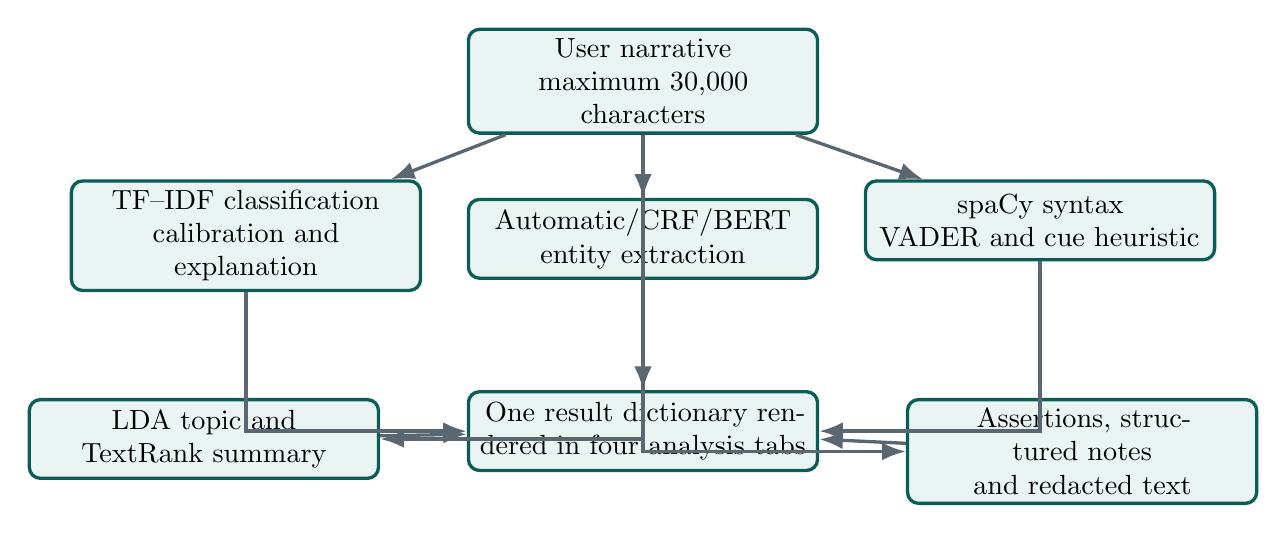
\begin{tikzpicture}[node distance=0.8cm]
  \node[flow] (input) {User narrative\\maximum 30,000 characters};
  \node[flow, below left=of input] (class) {TF--IDF classification\\calibration and explanation};
  \node[flow, below=of input] (entity) {Automatic/CRF/BERT\\entity extraction};
  \node[flow, below right=of input] (language) {spaCy syntax\\VADER and cue heuristic};
  \node[flow, below left=1.5cm and 1.1cm of entity] (topic) {LDA topic and\\TextRank summary};
  \node[flow, below right=1.5cm and 1.1cm of entity] (privacy) {Assertions, structured notes\\and redacted text};
  \node[flow, below=1.4cm of entity] (result) {One result dictionary rendered in four analysis tabs};
  \draw[arrow] (input) -- (class);
  \draw[arrow] (input) -- (entity);
  \draw[arrow] (input) -- (language);
  \draw[arrow] (class) |- (result);
  \draw[arrow] (entity) -- (result);
  \draw[arrow] (language) |- (result);
  \draw[arrow] (topic) -- (result);
  \draw[arrow] (privacy) -- (result);
  \draw[arrow] (input) |- (topic);
  \draw[arrow] (input) |- (privacy);
\end{tikzpicture}
\caption{On-demand analysis of one narrative.}
\end{figure}

The four tabs show entities and summary, syntax and morphology, evidence retrieval, and analysis details. Downloads include a JSON analysis, a redacted narrative and a page-limited CSV from search results.

\chapter{Scala, Cluster and Deployment Components}

\section{Scala functional-programming component}

\path{scala/CrimeAnalytics.scala} is a supplementary executable example for the Big Data syllabus. It demonstrates immutable values, a case class, a trait and object, pattern matching, closures, list/set/map collections and Dataset transformations. \path{scripts/run_scala.py} uses the Scala compiler distributed with PySpark, creates a JAR and submits it to Spark against the processed report Parquet.

The primary application remains Python; the Scala component demonstrates interoperability and functional concepts rather than reimplementing the dashboard.

\section{Standalone Spark launcher}

\path{scripts/run_cluster.py} starts a Spark master and two worker JVMs, waits until both register, runs the Spark pipeline against the standalone master, records worker metadata, and terminates only processes that it started. The saved receipt explicitly states that both workers ran on one Windows host.

\section{Container definitions}

The Dockerfile uses Python 3.12 slim and installs Java 17. Docker Compose defines the dashboard, Spark master, Spark worker and pipeline services. The dashboard binds to localhost port 8501. Cluster services are optional profile members. These definitions provide a deployment template, but the project's documentation does not claim that container execution was verified on the development machine.

\chapter{Artifacts and Inter-Module Linkage}

\section{How modules are connected}

\begin{longtable}{p{0.24\textwidth}p{0.30\textwidth}p{0.36\textwidth}}
\toprule
Producer & Artifact/interface & Consumer \\
\midrule
\endhead
\path{generate.py} & Raw JSONL and exact entity spans & \path{spark_pipeline.py} \\
\path{spark_pipeline.py} & Partitioned clean Parquet & \path{train.py}, \path{enrich.py}, Scala example \\
\path{train.py} & TF--IDF, BoW, Word2Vec, CRF, BERT and topic models & \path{enrich.py}, \path{inference.py}, dashboard evaluation pages \\
\path{train.py} & Calibration and selected-NER JSON & Enrichment and on-demand inference \\
\path{enrich.py} & Dashboard Parquet & Overview, filters, results table and topic pages \\
\path{enrich.py}/\path{store.py} & SQLite case database & Selected report retrieval and entity filters \\
\path{enrich.py} & Sparse TF--IDF matrix & Keyword and hybrid search \\
\path{enrich.py}/\path{semantic.py} & Dense MiniLM array & Semantic and hybrid search \\
\path{inference.py} & Unified result dictionary & Four dashboard analysis tabs and downloads \\
\path{evaluation.py} & Metrics and calibrated probabilities & Training artifacts and model-evaluation dashboard \\
\path{audit.py} & Stage signatures and output hashes & Safe pipeline resume and reproducibility receipts \\
\bottomrule
\end{longtable}

\section{Important artifact files}

\begin{itemize}
  \item \path{dataset_manifest.json}: corpus size, seed, categories, faults and split policy.
  \item \path{data_quality.json}: cleaning counts, schema, length quantiles and split/category counts.
  \item \path{spark_metrics.json}: Spark version, master, partitions, runtime and MLlib result.
  \item \path{evaluation_plan.json}: sample sizes, group separation and selection policy.
  \item \path{frozen_models.json}: SHA--256 fingerprints of model files before final evaluation.
  \item \path{evaluation.json}: document metrics, confusion matrices, bootstrap intervals and calibration.
  \item \path{ner_evaluation.json}: selected NER, both model results and per-entity metrics.
  \item \path{topics.json}: LDA terms, NMF terms, coherence, diversity and perplexity.
  \item \path{index_manifest.json}: search row-order fingerprint and embedding details.
  \item \path{final_evaluation_receipt.json}: proof that the final test followed model freezing.
\end{itemize}

\chapter{Testing and Reproducibility}

\section{Test coverage}

The test suite checks functionality rather than merely checking that files exist.

\begin{itemize}
  \item \textbf{Text tests:} offsets, BIO round trips, negation, extractive summaries, evidence abstention, HTML escaping and BIO repair.
  \item \textbf{Version-2 tests:} calibration normalization, review thresholds, redaction, hybrid retrieval, JSONL quarantine, feedback privacy, BERT windows and resume invalidation.
  \item \textbf{Artifact tests:} 60,000-row invariants, split separation, index order, valid entity spans, metric consistency and offline model inference.
  \item \textbf{Dashboard tests:} all pages, narrative analysis, empty search results, semantic/hybrid retrieval and pagination.
\end{itemize}

\section{Reproducibility mechanisms}

Reproducibility is supported by fixed seeds, explicit package constraints, a resolved lock file, centralized settings, local cached pretrained resources, deterministic sample ordering, training-only vectorizer fitting, validation-only selection, model hashes, stage receipts and saved metrics. Reproducibility does not mean numerical identity on every possible hardware/library combination, but these controls reduce avoidable variation.

\chapter{Measured Results}

\section{Data and model results}

\begin{table}[H]
\centering
\begin{tabular}{lr}
\toprule
Measurement & Recorded value \\
\midrule
Raw rows & 62,700 \\
Invalid rows removed & 1,200 \\
Duplicates removed & 1,500 \\
Clean reports & 60,000 \\
Spark MLlib accuracy & 87.49\% \\
Bag of Words accuracy & 78.42\% \\
TF--IDF accuracy & 83.67\% \\
Word2Vec accuracy & 95.17\% \\
BERT document accuracy & 83.25\% \\
Selected NER model & CRF \\
CRF strict entity F1 & 98.46\% \\
BERT strict entity F1 & 87.41\% \\
\bottomrule
\end{tabular}
\caption{Principal measurements from saved version-2 artifacts.}
\end{table}

The results must be interpreted together with the protocol. Word2Vec performed best for document classification in this experiment, while the classical CRF performed best for entity extraction. This is evidence for the particular synthetic corpus, sample sizes and hyperparameters; it is not a universal ranking of algorithms.

\chapter{Contributions to NLP and Big Data Learning}

\section{NLP contributions}

\begin{itemize}
  \item Demonstrates sparse lexical representations through BoW and TF--IDF.
  \item Demonstrates neural distributional representation through Word2Vec.
  \item Demonstrates contextual Transformer fine-tuning through BERT.
  \item Demonstrates structured sequence prediction through CRF and BIO tagging.
  \item Demonstrates unsupervised discovery through LDA and NMF.
  \item Demonstrates syntax, morphology and dependency relations with spaCy.
  \item Demonstrates rule/lexicon sentiment with VADER.
  \item Demonstrates graph-based extractive summarisation with TextRank.
  \item Demonstrates lexical, semantic and fused information retrieval.
  \item Demonstrates accuracy, precision, recall, F1, calibration, bootstrap intervals and confusion matrices.
\end{itemize}

\section{Big Data contributions}

\begin{itemize}
  \item Uses schema-driven Spark DataFrames and partitioned computation.
  \item Distinguishes transformations from actions and records a physical plan.
  \item Uses deterministic window-based deduplication and Spark SQL aggregation.
  \item Writes columnar Parquet partitioned by evaluation split.
  \item Executes a real MLlib Pipeline rather than only importing Spark.
  \item Demonstrates standalone master/worker processes on one host.
  \item Connects batch analytics storage with a transactional local query store.
  \item Preserves lineage using stable IDs, source fields, hashes and manifests.
\end{itemize}

\chapter{Limitations, Ethics and Future Work}

\section{Current limitations}

\begin{enumerate}
  \item The corpus is generated and lacks the ambiguity, diversity and annotation disagreement of real narratives.
  \item Shared generator grammar and vocabulary remain across evaluation partitions.
  \item The compact BERT classifier truncates document input after 160 subtokens.
  \item MiniLM retrieval truncates each indexed case after 128 subtokens.
  \item Search and evidence thresholds are heuristics, not calibrated relevance probabilities.
  \item Syntax, sentiment, threat cues, retrieval and summaries lack independent human-reference evaluation sets.
  \item Negation uses a small local window and can fail on complex language.
  \item Redaction can miss identifiers and must be reviewed before sharing.
  \item A single-host two-worker run does not demonstrate multi-machine scalability.
  \item Shared-password access and local SQLite storage are not production security architecture.
\end{enumerate}

\section{Ethical interpretation}

Suspect and victim labels identify linguistic roles in fictional allegations. They do not establish responsibility, truth or guilt. Synthetic trends must not be presented as real crime rates. Model predictions must not be used to rank individuals, predict criminality or automate consequential decisions.

\section{Recommended future work}

The most valuable next experiment is a permissioned, independently annotated dataset with double annotation, disagreement adjudication and a source-separated final test. Other useful work includes human relevance judgements for search, human summary evaluation, explicit redaction false-negative tests, multilingual evaluation, drift monitoring, calibrated entity confidence, approximate nearest-neighbour indexing and measured multi-host Spark throughput.

\chapter{Execution Guide}

\section{Fresh build}

The project expects Python 3.12 and Java 17. From the project directory:

\begin{lstlisting}[language=bash]
py -3.12 -m venv .venv312
.\.venv312\Scripts\python.exe -m pip install -r requirements.txt
.\.venv312\Scripts\python.exe scripts\download_resources.py
.\.venv312\Scripts\python.exe run_pipeline.py
.\.venv312\Scripts\python.exe -m pytest -q
.\.venv312\Scripts\python.exe -m streamlit run app.py
\end{lstlisting}

\section{Separate stages and alternatives}

\begin{lstlisting}[language=bash]
python run_pipeline.py --stage generate
python run_pipeline.py --stage spark
python run_pipeline.py --stage train
python run_pipeline.py --stage enrich
python run_pipeline.py --resume
python scripts\run_cluster.py
python scripts\run_scala.py
\end{lstlisting}

The dashboard should be stopped before rebuilding because it may hold cached resources or open files. If an upstream stage changes, downstream artifacts must be rebuilt unless hash-based resume proves them unchanged.

\chapter{Conclusion}

\project{} is not one isolated machine-learning script. It is a connected system in which each component has a defined responsibility. The generator supplies traceable labelled text; Spark produces reliable analytical data; training compares multiple representations and sequence models; evaluation controls model selection and records uncertainty; enrichment converts the corpus into searchable predictions; Parquet, SQLite and vector indexes support different access patterns; and Streamlit exposes the results with explanations and warnings.

Its principal academic contribution is the integration of NLP theory and Big Data engineering into a reproducible workflow. Its principal scientific limitation is equally clear: measured performance belongs to a synthetic benchmark and must not be treated as evidence of readiness for real policing or other consequential use.

\appendix
\chapter{Code Map}

\begin{longtable}{p{0.35\textwidth}p{0.55\textwidth}}
\toprule
File or directory & Responsibility \\
\midrule
\endhead
\path{settings.toml} & Seeds, sample sizes, thresholds and Spark defaults. \\
\path{run_pipeline.py} & Stage orchestration, arguments and run status. \\
\path{crime_nlp/generate.py} & Synthetic corpus and exact spans. \\
\path{crime_nlp/corpus_patterns.py} & Layout and participant phrase families. \\
\path{crime_nlp/spark_pipeline.py} & Spark cleaning, SQL, Parquet and MLlib. \\
\path{crime_nlp/train.py} & Classical models, Word2Vec, topics and evaluation protocol. \\
\path{crime_nlp/bert_model.py} & BERT document classifier. \\
\path{crime_nlp/ner_model.py} & BERT token classifier and long-text windows. \\
\path{crime_nlp/evaluation.py} & Metrics, calibration and BIO repair. \\
\path{crime_nlp/enrich.py} & Full-corpus predictions and index construction. \\
\path{crime_nlp/inference.py} & Unified analysis of one narrative. \\
\path{crime_nlp/text.py} & Tokenisation, CRF features, TextRank and cue heuristic. \\
\path{crime_nlp/topics.py} & Lemma-based topic preprocessing. \\
\path{crime_nlp/semantic.py} & MiniLM embeddings, search fusion and cited evidence. \\
\path{crime_nlp/store.py} & SQLite cases, feedback and audit events. \\
\path{crime_nlp/privacy.py} & Assertions, structured summaries and redaction. \\
\path{crime_nlp/audit.py} & Stage signatures, hashes and resume validation. \\
\path{crime_nlp/import_data.py} & External JSONL validation and quarantine. \\
\path{app.py} & Streamlit pages, controls, charts and interactions. \\
\path{scala/CrimeAnalytics.scala} & Scala and Spark Dataset exercise. \\
\path{tests/} & Unit, integration, privacy, artifact and dashboard tests. \\
\path{artifacts/} & Metrics, manifests, receipts, indexes and model evidence. \\
\bottomrule
\end{longtable}

\chapter{Glossary}

\begin{longtable}{p{0.25\textwidth}p{0.65\textwidth}}
\toprule
Term & Meaning \\
\midrule
\endhead
Corpus & A collection of text documents. \\
Feature & A numeric signal supplied to a machine-learning model. \\
Label & The reference answer a supervised model learns to predict. \\
Embedding & A dense vector representation of a word, sentence or document. \\
Inference & Applying a trained model to new input. \\
Epoch & One complete pass through the training examples. \\
Checkpoint & Saved model parameters from a particular training point. \\
Calibration & Alignment between model confidence and observed correctness. \\
Named Entity Recognition & Identification and typing of spans inside text. \\
Partition & A portion of a dataset processed as a Spark task unit. \\
Parquet & A compressed, column-oriented analytical storage format. \\
Data leakage & Evaluation information influencing training or model selection. \\
Provenance & Evidence describing where data came from and how it was processed. \\
Hash & A deterministic content fingerprint used to detect changes. \\
\bottomrule
\end{longtable}

\end{document}
